\section{Monolithic Architecture}

\begin{frame}{Monolithic Architecture}
    \begin{itemize}
        \item Monolith ist altgriechisch für \textit{einheitlicher Stein}
        \item Einheitlich: Alles ist eins - alle Funktionalitäten in einer Komponente
        \item Stein: Altes Material - früher gut. Heute schlecht?
        \item Problem: Enge Kopplung
    \end{itemize}
\end{frame}

\begin{frame}{Monolithic Architecture: Beispiel E-Commerce}
    \begin{figure}[!h]
        \centering
        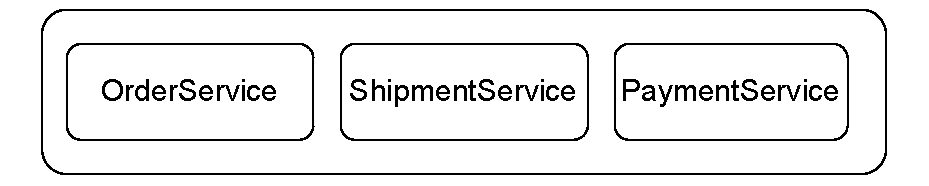
\includegraphics[scale=0.70]{imglib/mono/mono}
        \caption{E-Commerce-Beispiel mit Monolithic Architecture}
        \label{fig:mono-ecommerce}
    \end{figure}
\end{frame}

\begin{frame}{Monotlithic Architecture: Agilität}
    \begin{itemize}
        \item Enge Kopplung ist fatal
        \begin{itemize}
            \item Keine kleinen autonomen Teams
            \item Erhöhte Komplexität und schwere Wartung $\Rightarrow$ längere Iterationen $\Rightarrow$ unflexibel
            \item Funktionalitäten nicht wiederverwendbar $\Rightarrow$ Mehraufwand \& Duplikation $\Rightarrow$ Änderungen teuer
            \item Isolierte Funktionstests sind möglicherweise aufwendig
        \end{itemize}
        \item Auslieferung nur im Ganzen \& längere Iterationen $\Rightarrow$ seltene Auslieferung
        \item Verpflichtung auf genau eine Technologie
        \item Horizontale Skalierung kaum möglich
        \item Aber: System ist nicht verteilt $\Rightarrow$ Keine Intersystemkommunikation $\Rightarrow$ Geringe Time-to-Market \& möglicherweise einfache System-Tests
    \end{itemize}
\end{frame}